\documentclass[12pt,a4paper]{report}
%\usepackage{charter}
\usepackage[latin1]{inputenc}
\usepackage[left=1.50cm, right=1.50cm, top=1.20cm]{geometry}
\renewcommand{\baselinestretch}{1.5}
\usepackage{listings}
\usepackage{xcolor}
\usepackage{graphicx}
\definecolor{listinggray}{gray}{0.9}
\definecolor{lbcolor}{rgb}{0.9,0.9,0.9}
\usepackage{float}
\usepackage{textcomp}
\lstdefinestyle{customc}{
	belowcaptionskip=1\baselineskip,
	aboveskip={1.2\baselineskip},
	breaklines=true,
	frame=lines,
	numbers=left,
	xleftmargin=\parindent,
	language=C++,
	showstringspaces=false,
	basicstyle=\sffamily,%,\ttfamily,
	keywordstyle=\bfseries\color{green!40!black},
	commentstyle=\itshape\color{purple!40!black},
	identifierstyle=\color{blue},
	stringstyle=\color{orange},
	breaklines=true,
	postbreak=\raisebox{0ex}[0ex][0ex]{\ensuremath{\color{red}\hookrightarrow\space}}
}

\lstdefinestyle{customasm}{
	belowcaptionskip=1\baselineskip,
	frame=L,
	xleftmargin=\parindent,
	language=[x86masm]Assembler,
	basicstyle=\footnotesize\ttfamily,
	commentstyle=\itshape\color{purple!40!black},
}
\lstset{escapechar=@,style=customc}

% Title Page
\title{Reading Notes: Multicore Application Programming: Windows, Linux and Oracle Solaris}


\begin{document}
\maketitle

\section*{Chapter 8}
\subsection*{Atomic Operations}
On x86 processors, the xadd instruction can be combined with the lock prefix to produce an atomic add, or the inc instruction can be combined with the lock prefix to produce an atomic increment.
\begin{lstlisting}
int atomic_add_int( volatile int *address, int value )
{
	asm volatile( "lock xadd %0,%1":
					"+r"(value):
					"+m"(*address):
					"memory" 
				);
	return value;
}
int atomic_inc_int( int *address )
{
	asm volatile ( "lock inc %0": :
					"+m"(*address):
					"memory" 
				);
	return (*address);
}
\end{lstlisting}
\begin{itemize}
	\item The keyword \textbf{asm} identifies the following text as an assembly language statement that will be inlined directly into the code. 
	\item he keyword \textbf{volatile} tells the compiler not to move the statement from where it has been placed, because such movement could cause a difference to the statement's semantics.
	\item The assembly language code is enclosed in the parentheses. There are multiple parts to the code. The first item in the parentheses, surrounded by quotes, is the instruction. The instruction uses virtual registers \%0 and \%1 as parameters. The compiler will allocate real registers later and will be responsible for populating these registers with the appropriate values.
	\item After the assembly language instruction, there are up to three colon-delimited lists. 
	\begin{itemize}
		\item The first list is of output variables and whether these are accesses to registers or memory. In the example, the expression ``+r''(value) means that the output parameter is a register that should be used to update the variable value. The plus sign means that the register will be both read and written by the instruction.
		\item 	The second list contains the input values and where these are located. Both routines take the pointer address as an input value, and the expression ``+m''(*address) indicates that this pointer is used as a memory access. The plus sign indicates that the instruction will both read and write the location in memory.
		\item The third list is the ``clobber'' list indicating what the instruction will modify. In both instances, the instruction will modify memory.
	\end{itemize}
	\item The virtual registers are numbered from the input registers, so register \%0 is assigned the value of the variable address. The output registers are the next set of virtual registers, so the variable value gets assigned to register \%1.
\end{itemize}
\subsubsection*{CAS Operation}
The CAS instruction can also be used in situations where atomic modification of an unusual variable type is required.
\begin{lstlisting}
void atomic_add_float( volatile float * variable, float increment )
{
	union
	{
		int asint;
		float asfp;
	} oldvalue, newvalue;
	
	do
	{
		oldvalue.asfp = *variable;                  // Line 11
		newvalue.asfp = oldvalue.asfp + increment;  // Line 12
	}
	while ( CAS( variable, oldvalue.asint, newvalue.asint ) != oldvalue.asint );
}
\end{lstlisting}
\begin{itemize}
	\item The code reads the value of the \textit{variable} to be modified and then prepares the modified version of this variable. 
	\item The \textit{variable} is read only once, at line 11, and then held in the local variable \textit{oldvalue}. This is to avoid a \textbf{data race} where the value changes between the first read of the variable and its use as one operand in the addition, at line 12. The race is subtle.
	\begin{itemize}
		\item Suppose that the first time the \textit{variable} is read, at line 11, it has the value 20; this is recorded as the original value of the variable. At this point, another thread changes the value of the variable, so the second time it is read, at line 12, it has the value 21. The value 21 is incremented to 22, and this will become the new value of the variable if the operation is successful.
		\item Suppose now that the other thread has returned the value of the variable to 20 by the time the CAS operation is tried. Since the variable contains 20 and this is the expected value, the CAS operation will store the value 22 into the variable, rather than the correct value of 21.
	\end{itemize} 
\end{itemize}
We can explore this problem of reloading values with another example.
\begin{lstlisting}
void addelement( element_t ** head, int value )
{
	element_t * element = (element_t*)malloc(sizeof(element_t));
	element->value = value;
	while (element!=0)
	{
		element->next = *head;
		if ( CAS( head, element->next, element ) == element->next)
	{
		element = 0;
	}
}
\end{lstlisting}
The code creates a new \textit{element} and stores the appropriate value in this. 
\begin{itemize}
	\item The loop keeps attempting to add this new element to the front of the list until it succeeds. 
	\item Each iteration of the loop sets the next field of the new element to be the next element in the list and then attempts to atomically compare and swap the head of the list with a pointer to the new element. 
	\item If the compare and swap succeeded, the return value will be the pointer to the element that used to be the top of the list. If this happens, the code has succeeded, and the loop can exit.
\end{itemize}
The problem with this code is that the \textbf{CAS()} function call causes the compiler to reload the value of \textbf{element\textrightarrow next}. 
\begin{itemize}
	\item There is a short window of opportunity for another thread to take the top element from the list between the \textbf{CAS()} function call and the load of \textbf{element\textrightarrow next}. 
	\item If this other thread takes the element off the list and modifies the value of \textbf{element\textrightarrow next}, then the compare and swap will not match with the new value of \textbf{element\textrightarrow next}, and the loop will assume that it failed to add the element to the queue, even though it actually succeeded. So, the code will attempt to add the element a second time, causing an error.
\end{itemize}
The solution is to hold the original value of *head in a local variable and use this in the comparison to determine whether the compare and swap was successful. 
\par
\textbf{Notice:}
cppreference.com give the following example:
\begin{lstlisting}
#include <atomic>
template<typename T>
struct node
{
	T data;
	node* next;
	node(const T& data) : data(data), next(nullptr) {}
};

template<typename T>
class stack
{
	std::atomic<node<T>*> head;
public:
void push(const T& data)
{
	node<T>* new_node = new node<T>(data);

	// put the current value of head into new_node->next
	new_node->next = head.load(std::memory_order_relaxed);

	// now make new_node the new head, but if the head
	// is no longer what's stored in new_node->next
	// (some other thread must have inserted a node just now)
	// then put that new head into new_node->next and try again
	while(!head.compare_exchange_weak(new_node->next, new_node,
	std::memory_order_release,
	std::memory_order_relaxed))
	; // the body of the loop is empty

// Note: the above use is not thread-safe in at least 
// GCC prior to 4.8.3 (bug 60272), clang prior to 2014-05-05 (bug 18899)
// MSVC prior to 2014-03-17 (bug 819819). The following is a workaround:
//      node<T>* old_head = head.load(std::memory_order_relaxed);
//      do {
//          new_node->next = old_head;
//       } while(!head.compare_exchange_weak(old_head, new_node,
//                               std::memory_order_release,
//                               std::memory_order_relaxed));
}
};
int main()
{
	stack<int> s;
	s.push(1);
	s.push(2);
	s.push(3);
}
\end{lstlisting}
\subsubsection*{Memory Order}
When a thread running on a multithread system performs a memory operation, that operation may or may not become visible to the rest of the system in the order in which it occurred.
\par
For example, an application might perform two store operations. On some processors, the second store operation could become visible to other processors before the first store operation becomes visible. This is called \textbf{weak memory ordering}.
\par
The kinds of memory barriers available are defined by the architecture. The x86 architecture defines the following:
\begin{itemize}
	\item \textbf{mfence}. Ensures that all previous loads and stores are visible to the system before any future loads and stores become visible.
	\item \textbf{sfence}. Ensures that all previous stores are visible to the system before any future stores become visible.
	\item \textbf{lfence}. Ensures that all previous loads are visible to the system before any future loads become visible
\end{itemize}
\paragraph*{Reordering by Compiler}
It is often thought that the \textbf{volatile} keyword provides a safety net that stops the compiler from optimizing code. Unfortunately, this is not true.
\par
The \textbf{volatile} keyword determines that the compiler needs to reload data from memory when it needs to use it and should store it back to memory as soon as it is modified. It does not stop the compiler from performing optimizations around the data nor does it form any kind of protection against data races.
\par
However, the \textbf{volatile} keyword is necessary to avoid the compiler optimizing away accesses to a variable.
\begin{lstlisting}
volatile int start;

void waitforstart()
{
	while( start == 0 ) {}
}
\end{lstlisting}
The variable \textit{start} is declared as \textbf{volatile}. If this were not the case, then the compiler would determine that the loop was either not entered or entered and infinite.
\begin{lstlisting}
volatile int count;

int* getnextelement()
{
	int element = 0;
	while( element == 0 )
	{
		if (count>0)
		{
			element = getElementFromList();
		}
	}
	return element;
}
\end{lstlisting}
In this case, the code contains a function call. Function calls, generally, cause the compiler to reload global data. However, if the variable \textit{count} is not declared to be \textbf{volatile}, it is still possible for the compiler to generate an infinite loop. 
\begin{itemize}
	\item The reason for this is that if \textit{count} does equal zero and it is not a \textbf{volatile} variable, then the call to \textit{getElementFromList()} will not be made, and the variable will remain zero. An optimizing compiler may identify this situation and replace the \textbf{else} branch of the \textbf{if} statement with an infinite loop.
\end{itemize}
\begin{lstlisting}
#include <stdio.h>
#include <pthread.h>

volatile int start[4];
volatile int done[4];

void * work( void* param )
{
	int id = (int)param;
	while ( start[id] == 0 ) {}
	printf( "Thread %i started\n", id );
	double total=0;
	for ( int i=0; i<100000000; i++ ) { total += i; }
	printf( "Thread %i done\n", id );
	done[id] = 1;
}
int main()
{
	pthread_t thread[4];
	for ( int i=0; i<4; i++ )
	{
		pthread_create( &thread[i], 0, work, (void*)i );
		done[i]=0;
	}
	for ( int i=0; i<4; i++ )
	{
		start[i] = 1;
	}
	for ( int i=0; i<4; i++ )
	{
		while( done[i] == 0 ){}
	}
	for ( int i=0; i<4; i++ )
	{
		pthread_join( thread[i], 0 );
	}
}
\end{lstlisting}
In this case,  the compiler can merge two loops, resulting in a change of behavior.
\begin{itemize}
	\item The code creates four threads. Each thread runs the same routine that prints out a statement that the thread is ready and then waits on the \textbf{volatile} variable \textit{start}.
	\item When the thread is started, it prints out a message before completing a short amount of work, printing a message indicating that it has completed its work and exiting.
	\item The main code creates the threads and, once all the threads are created, signals to the threads that they can start working. Once this has been done, it waits for all the threads to complete their work, before calling \textit{pthread\_join()} on each of the threads.
\end{itemize}
When compiled \textbf{without optimization}, all the threads proceed at the same time, so the output from the application shows all the threads starting and then all the threads completing. 
\par
When compiled \textbf{with optimizatio}n, the threads are \textbf{serialized}, so each thread prints the message that it has started followed by the message that it has completed.
\begin{lstlisting}
$ cc loop_merge.c
$ ./a.out
	Thread 1 started
	Thread 2 started
	Thread 0 started
	Thread 3 started
	Thread 1 done
	Thread 0 done
	Thread 2 done
	Thread 3 done
$ cc -O loop_merge.c
$ ./a.out
	Thread 0 started
	Thread 0 done
	Thread 1 started
	Thread 1 done
	Thread 2 started
	Thread 2 done
	Thread 3 started
	Thread 3 done
\end{lstlisting}
With optimization, the compiler has merged the code in the two loops that set the start variable and read the end variable. This produces code similar to that shown in the following.
\begin{lstlisting}
int main()
{
	pthread_t thread[4];
	for( int i=0; i<4; i++ )
	{
		pthread_create( &thread[i], 0, work, (void*)i );
		done[i] = 0;
	}
	for ( int i=0; i<4; i++ )
	{
		start[i] = 1;
		while( done[i] == 0 ){}
	}
	for ( int i=0; i<4;i++ )
	{
		pthread_join( thread[i], 0 );
	}
}
\end{lstlisting}
The two loops contain no function calls, and the compiler considers the accesses to the volatile variables to be without side effects. Hence, the compiler considers it safe to merge the two loops.
\par
To correct this situation, we need to modify the code so that the compiler is unable to merge the two loops.
\begin{itemize}
	\item The easiest way to do this is to place a\textbf{ function call} either in one of the loops or between the two loops.
	\item An alternative approach would be to separate the two loops with serial code that is unable to be moved because of some dependency or potential aliasing issue.
\end{itemize}
However, both of these approaches will add some unnecessary instructions into the code, and both approaches run the risk that a ``smart'' compiler might identify the instructions as unnecessary and remove them.
\par
The good slution is to use a \textbf{gcc asm("":::"memory")} construct that cause the compiler to correctly order the loops. This statement stops the loops from merging and adds no additional instructions into the code.
\begin{lstlisting}

int main()
{
	pthread_t thread[4];
	for ( int i=0; i<4; i++ )
	{
		pthread_create( &thread[i], 0, work, (void*)i );
		done[i] = 0;
	}
	for ( int i=0; i<4; i++ )
	{
		start[i] = 1;
	}

	asm volatile( "": : : "memory" );
	for ( int i=0; i<4; i++ )
	{
		while( done[i] == 0 ){}
	}
	for ( int i=0; i<4;i++ )
	{
		pthread_join( thread[i], 0 );
	}
}

\end{lstlisting}
Windows provides intrinsics for this purpose. The functions \textbf{\_ReadBarrier()}, \textbf{\_WriteBarrier()}, and \textbf{\_ReadWriteBarrier()} are defined in \textbf{intrin.h}. These intrinsics tell the compiler not to reorder the operations.
\begin{itemize}
	\item A \textbf{\_ReadBarrier()} call ensures that all reads will have completed at that point
	\item A \textbf{\_WriteBarrier()} call ensures that all writes have completed
	\item These instructions only enforce the compiler ordering and do not generate any instructions.
\end{itemize}
\paragraph*{Volatile Variables}
Using the \textbf{volatile} keyword is necessary to avoid undesirable \textbf{caching}, in registers, of the values held in memory locations. However, the keyword also stops desirable caching of the variable, so any use of the variable can be \textbf{expensive}.
\par
However, it should be observed that use of compiler memory barriers can be \textbf{low cost} and a more accurate way of ensuring that variables are stored back to memory and reloaded from memory at the desired point in the code.
\begin{lstlisting}
extern int start;

void waitforstart()
{
	while(start==0) { asm volatile( "": : : "memory" ); }
}

\end{lstlisting}
This case avoid having to declare the variable \textit{start} as \textbf{volatile} and instead uses a \textbf{compiler barrier} to ensure that the value is reloaded from memory.
\subsection*{Lock--Free Algorithms}
\begin{lstlisting}
volatile int priority = 0;
volatile int counter = 0;
volatile int waiting[2];

void increment( int id )
{
	waiting[id] = 1;

	while( waiting[1-id] == 1 )
	{
		if ( priority != id )
		{
			waiting[id] = 0;
			while ( priority != id ){}
			waiting[id] = 1;
		}
	}
	/* Critical section */
	counter++;
	/* Exit critical section */
	priority = 1-id;
	waiting[id] = 0;
}
\end{lstlisting}
\subsubsection*{Dekker's Algorithm}
The algorithm works because each thread signals that it is waiting to get into the critical section. If the other thread has not signaled that it is waiting for or has already entered the critical section, then the current thread can enter it. If both threads are waiting, then one of the threads gets priority, and the other thread waits until it gets \textit{priority}.
\\
The problem with the code is one of memory ordering.
\begin{itemize}
	\item The two threads can simultaneously indicate that they are waiting to enter the critical section by storing to their index in the waiting array.
	\item In the very next cycle (i.e. when both threads running to \textbf{line 9}), they load the other thread's waiting status. Since the other thread has only just issued the store, the \textbf{store} has not yet made its way through the pipeline to be visible to the rest of the system.
	\item So, the load instruction picks up a zero, indicating that the other thread is not waiting for the critical section. 
	\item Both threads fail to see the other thread waiting, and both threads enter the critical region.
\end{itemize}
The way to fix this is to put memory barriers into the code.
\begin{itemize}
	\item The memory barriers ensure that previous memory operations have completed before the next memory operation issues.
	\item In this case, we want to ensure that the \textbf{store} to indicate a thread is waiting is completed \textbf{before} the \textbf{load} to check whether the other thread is also waiting.
	\item Consider the sequence of operations. Both threads hit the \textbf{store} at the same time; both threads now wait until the \textbf{stores} are \textbf{visible} to the other processor before issuing their load. So, both threads will get the data that was stored by the other thread.
\end{itemize}
On \textbf{x86} processors, it is necessary to use an \textbf{mfence} operation that ensures that all previous memory operations complete before the next memory operation is issued.
\begin{lstlisting}
#include <stdio.h>
#include <pthread.h>

volatile int priority = 0;
volatile int counter = 0;
volatile int waiting[2];

void increment( int i )
{
	waiting[i] = 1;

	#ifdef __sparc
		asm( "membar #StoreLoad": : : "memory" );
	#else
		asm( "mfence": : : "memory" );
	#endif
	
	while( waiting[1-i] == 1 )
	{
		if ( priority != i )
		{
			waiting[i] = 0;
			while ( priority != i ){}
			waiting[i] = 1;
			#ifdef __sparc
				asm( "membar #StoreLoad": : : "memory" );
			#else
				asm( "mfence": : :"memory" );
			#endif
		}
	}

	counter++;
	priority = 1-i;
	waiting[i] = 0;
}
\end{lstlisting}
\subsubsection*{Producer--Consumer with a Circular Buffer}
Consider the case where there is a producer-consumer pair of threads that communicate through a circular buffer. It is possible to write code that does not require locks or atomic operations to handle this situation.
\begin{lstlisting}
#include <stdio.h>
#include <pthread.h>
#include <stdlib.h>

volatile int volatile buffer[16];
volatile int addhere;
volatile int removehere;

void clearbuffer()
{
	addhere = 0;
	removehere = 0;
	for( int i=0; i<16; i++ ) { buffer[i] = 0; }
}

int next( int current )
{
	return ( current+1 ) & 15;
}

void addtobuffer( int value )
{
	while( next(addhere) == removehere ) {} // Spin waiting for room
	if ( buffer[addhere] != 0 )
	{ printf( "Circular buffer error\n" ); exit(1); }
	buffer[addhere] = value;                // Add item to buffer
	addhere = next(addhere);                // Move to next entry
}

int removefrombuffer()
{
	int value;
	while( ( value = buffer[removehere] ) == 0 ){} // Spin until
	// something in buffer
	buffer[removehere] = 0;                        // Zero out element
	removehere = next(removehere);                 // Move to next entry
	return value;
}
\end{lstlisting}
There are actually two implicit constraints that ensure that the code works. One constraint is that stores and loads are themselves atomic. The other constraint is that stores do not become reordered.
\\
The requirement for ordering stores comes from the code that removes elements from the array.
\begin{itemize}
	\item The location containing the element to be removed is zeroed out, then the pointer to the end element to be removed is advanced to the next location in the array.
	\item If these actions became visible to the producer thread in the \textbf{wrong order}, the producer thread would see that the end pointer had been advanced. This would allow it to enter the code that adds a new element.
	\item However, the first test this code performs is to check that the new location is really empty. If the store of zero to the released array position was delayed, this location would still contain the old value, and the code would exit with an error. The check validates that the code is behaving correctly.
\end{itemize}
Several characteristics of the algorithm enable it to work correctly.
\begin{itemize}
	\item There are 2 pointers that point to locations in the array. Only one thread is responsible for updating each of these variables. The other thread only reads the variable.
	\item As long as the \textbf{reading thread} sees the updates to memory in the correct order and each variable is updated \textbf{atomically}, the thread will continue to wait until the data is ready and only then read that data.
	\item The updates of the pointers into the array are carried out by a \textbf{function call}. The function call acts as a \textbf{compiler memory barrier} and forces the compiler to store variables back to memory. Otherwise, there would be the risk that the compiler might reorder the store operations.
\end{itemize}
\subsubsection*{Scaling the Producer-Consumer to Multiple Threads}
The simplest way to share the circular buffer between threads would be to use some kind of mutual exclusion that would ensure that only a single thread at a time could modify the structure. 
\begin{lstlisting}
#include <stdio.h>
#include <pthread.h>

volatile int volatile buffer[16];
volatile int addhere;
volatile int removehere;
volatile int lock = 0;

void lock_spinlock( volatile int* lock )
{
	while ( CAS( lock, 0, 1 ) != 0 ) {}
	acquire_memory_barrier();
}

void free_spinlock( volatile int *lock )
{
	release_memory_barrier();
	*lock = 0;
}
void clearbuffer()
{
	addhere = 0;
	removehere = 0;
	for( int i=0; i<16; i++ ) { buffer[i] = 0; }
}

int next( int current )
{
	return ( current + 1 ) & 15;
}
void addtobuffer( int value )
{
	lock_spinlock( &lock );
	while( buffer[ next(addhere) ] != 0 ) {}
	buffer[addhere] = value;
	addhere = next(addhere);
	free_spinlock( &lock );
}

int removefrombuffer()
{
	int value;
	lock_spinlock( &lock );
	while( ( value = buffer[removehere] ) == 0 ){}
	buffer[removehere] = 0;
	removehere = next(removehere);
	free_spinlock( &lock );
	return value;
}
\end{lstlisting}
The code now contains a deadlock. Imagine that the circular buffer is empty and a consumer thread acquires the lock and starts waiting for something to appear in the buffer. A producer thread eventually arrives but now has to acquire the lock before it can add anything into the buffer. Both threads end up spinning, waiting for an event that can never happen.
\\
There are 2 solutions to this particular instance of the problem.
\\
One solution is to provide two locks---one for threads waiting to add elements to the buffer and the second for threads waiting to remove an item from the list. This solution works in this situation because it reduces the problem down to the one described earlier where there are only two threads present in the system.
\begin{itemize}
	\item 	One lock ensures that only one producer thread can access the circular buffer at a time. 
	\item The other lock ensures that only one consumer thread can access the circular buffer at a time.
	\item The other producer and consumer threads cannot interfere and cause correctness problems.
\end{itemize}
Another solution uses only one single lock. One way of doing this is to place the critical section inside another loop, which repeats the loop until the critical section is successfully executed. This requires modification to the \textbf{addtobuffer()} and \textbf{removefrombuffer()} routines so that they no longer loop inside the critical section and instead quickly return success or failure.
\begin{lstlisting}
void addtobuffer( int value )
{
	int success = 0;
	while( !success )
	{
		lock_spinlock( &lock );
		if( buffer[ next(addhere) ] == 0 )
		{
			buffer[addhere] = value;
			addhere = next(addhere);
			success = 1;
		}
		free_spinlock( &lock );
	}
}

int removefrombuffer()
{
	int value;
	int success = 0;
	while ( !success )
	{
		lock_spinlock( &lock );
		if ( ( value = buffer[removehere] ) != 0 )
		{
			buffer[removehere] = 0;
			removehere = next(removehere);
			success = 1;
		}
		free_spinlock( &lock );
	}
	return value;
}
\end{lstlisting}
The code uses a variable \textit{success} to determine whether the critical region was successful. Although this change results in the desired behavior for the code, it is not the best code to run on the system. The problem with the code is that while threads are unable to add or remove items from the queue, the spinlock is constantly being acquired and released.
\begin{itemize}
\item This results in significant traffic between the cores invalidating and fetching the cache line containing the lock variable.
\item Both the acquisition and release of the variable lock result in a store operation, which causes all the other caches to invalidate the cache line containing the lock.
\item When the next thread acquires the spinlock, it has to fetch it from the cache of the processor that last updated the lock.
\item This activity causes the cache line containing the variable lock to be constantly being passed between the caches of different virtual CPUs and may have an impact on the performance of the system.
\end{itemize}
One way of improvement is to add a test success in accessing the buffer before acquiring the lock.
\begin{lstlisting}
void addtobuffer( int value )
{
	int success = 0;
	while ( !success )
	{
		if ( buffer[ next(addhere) ] == 0 ) // Wait for an empty space
		{
			lock_spinlock( &lock );
			if( buffer[ next(addhere) ] == 0 )
			{
				buffer[addhere] = value;
				addhere = next(addhere);
				success = 1;
			}
			free_spinlock( &lock );
		}
	}
}

int removefrombuffer()
{
	int value;
	int success = 0;
	while ( !success )
	{
		if ( buffer[removehere] != 0 ) // Wait for an item to be added
		{
			lock_spinlock( &lock );
			if ( ( value = buffer[removehere] ) != 0 )
			{
				buffer[removehere] = 0;
				removehere = next(removehere);
				success = 1;
			}
			free_spinlock( &lock );
		}
	}
	return value;
}
\end{lstlisting}
\begin{itemize}
		\item This test for success is to load the next element in the buffer array and see whether it is zero. 
		\item The advantage of using \textbf{load} instructions is that the cache line fetched by a load remains resident in cache until it is invalidated by a store operation.
		\item In practical terms, each thread will spin on the appropriate variable waiting for it to be modified. This causes \textbf{no invalidation} of the values held in other caches until the variable is actually updated.
		\item Consequently, there is little risk of there being a performance impact from this scheme.
\end{itemize}
The problem with this code is that every time a new item is added to the circular buffer or every time a space becomes free, all the waiting threads recognize this and attempt to acquire the lock, even though only one thread can actually succeed.
\\
This is an example of the \textbf{thundering herd problem} where a number of threads are waiting for a condition to become true and \textbf{only one thread can successfully proceed}, so all the other threads end up using unnecessary resources. This problem can be resolved by \textbf{ordering} the list of threads such that only one thread is allowed to proceed.
\\
However, the problem is worse than this. All the threads that identify the opportunity to access the circular buffer will enter the \textbf{if} statement and can exit only after they have acquired and released the spinlock. So, these threads will end up spinning on the spinlock, which was not the intention of the code.
\\
To remove this problem, we should change the code so that instead of spinning on the spinlock, the threads try to acquire it, and if they do not, then they should return to the outer loop and wait for the next opportunity to access the circular buffer.
\begin{lstlisting}
int try_spinlock( volatile int* lock )
{
	if ( CAS( lock, 0, 1 ) == 1 ) { return 0; }
	else
	{
		acquire_memory_barrier();
		return 1;
	}
}

void addtobuffer( int value )
{
	int success = 0;
	while ( !success )
	{
		if ( buffer[ next(addhere) ] == 0 )
		{
			if (try_spinlock( &lock ) )
			{
				if ( buffer[ next(addhere) ] == 0 )
				{
					buffer[addhere] = value;
					addhere = next(addhere);
					success = 1;
				}
				free_spinlock( &lock );
			}
		}
	}
}

int removefrombuffer()
{
	int value;
	int success = 0;
	while ( !success )
	{
		if ( buffer[removehere] != 0 )
		{
			if ( try_spinlock( &lock ) )
			{
				if ( ( value = buffer[removehere] ) !=0 )
				{
					buffer[removehere] = 0;
					removehere = next(removehere);
					success = 1;
				}
				free_spinlock( &lock );
			}
		}
	}
	return value;
}
\end{lstlisting}
It introduces a function called \textbf{try\_spinlock()} that will either \textbf{acquire} the \textbf{spinlock} and return \textbf{true} or \textbf{fail} to acquire the lock and return \textbf{false}. With this modification, 
\begin{itemize}
\item the threads spin on the variable, indicating the state of the circular buffer. 
\item This variable is shared so it does not produce much memory traffic. 
\item If the state changes, the threads attempt to get the spinlock.
\item Only one thread will succeed, and this thread gets to access the buffer while the other threads go back to spinning on the shared variable.
\end{itemize}
With this change, the \textbf{spinlock} has ceased to be used as a spinlock since the threads spin before attempting to acquire the lock.
\\
We can make further improvement to reduce the number of CAS operations, we could spins until the lock has been \textbf{acquired} by the calling thread.
\begin{lstlisting}
void lock_spinlock( volatile int* lock )
{
	int acquired = 0;
	while ( !acquired )
	{
		if ( ( *lock == 0 ) && ( CAS( lock, 0, 1 ) == 0) )
		{
			acquired = 1;
		}
	}
	acquire_memory_barrier();
}

void addtobuffer( int value )
{
	int success = 0;
	while ( !success )
	{
		if ( buffer[ next(addhere) ] == 0 )
		{
			lock_spinlock( &lock );
			if ( buffer[ next(addhere) ] == 0 )
			{
				buffer[addhere] = value;
				addhere = next(addhere);
				success = 1;
			}
			free_spinlock( &lock );

		}
	}
}

int removefrombuffer()
{
	int value;
	int success = 0;
	while ( !success )
	{
		if ( buffer[removehere] != 0 )
		{
			lock_spinlock( &lock );
			if ( ( value = buffer[removehere] ) !=0 )
			{
				buffer[removehere] = 0;
				removehere = next(removehere);
				success = 1;
			}
			free_spinlock( &lock );
		}
	}
	return value;
}
\end{lstlisting}
In each iteration, the loop tests whether the lock is available. If the lock is available, the code attempts to acquire the lock atomically. If successful, the code \textbf{exits} the loop having acquired the spinlock. If unsuccessful, the loop continues to spin.

\subsubsection*{Modifying the Producer-Consumer Code to Use Atomics}
\begin{lstlisting}
void addtobuffer( int value )
{
	int success = 0;
	while ( !success )
	{
		if ( buffer[ next(addhere) ] == 0 )
		{
			if ( CAS( &buffer[ next(addhere) ], 0, value ) == 0 )
			{
				addhere = next(addhere);
				success = 1;
			}
		}
	}
}

int removefrombuffer()
{
	int value;
	int success = 0;
	while ( !success )
	{
		if ( ( value = buffer[removehere] ) != 0 )
		{
			if ( CAS( &buffer[removehere], value, 0 ) == value )
			{
				removehere = next(removehere);
				success = 1;
			}
		}
	}
	return value;
}

\end{lstlisting}
It appears that this should work. Only one thread at a time can successfully add or remove an element. Only that thread will alter the pointer so that it points to the next entry.However, this is not the case.
\\
It is critical to realize that although instructions will execute in the expected order, the gaps between the execution of adjacent instructions are random. A pair of instructions could be executed on the same cycle or with a separation of only a few cycles.
\\
However, a thread may be \textbf{context switched off} the virtual CPU between the two instructions, and this would cause a gap of thousands of cycles to occur between the two operations.
\\
Consider the situation shown in following figure where multiple producer and consumer threads exist.
\begin{center}
	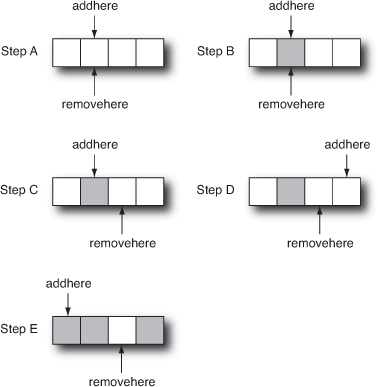
\includegraphics{multicore_getfile.jpg}
\end{center}
\begin{itemize}
\item  At \textbf{step A}, two producer threads are attempting to add an item into the circular buffer. They both reach the \textbf{CAS} instruction at nearly the same time, but one of the threads gets context switched off the CPU at that very moment.
\item At \textbf{step B}, the other thread successfully enters its value into the circular list and is just about to move the \textbf{addhere} pointer onto the next element when it too is context switched off the virtual CPU.
\item At\textbf{ step C}, while the first thread is off-processor, one of the consumer threads come along and removes the recently inserted element. At that point, the first thread is switched back onto the CPU, and it sees that the slot it was planning to use is now empty. It atomically inserts its item of data into the circular buffer and then increments the pointer to the next place to insert an element.
\item This is rapidly followed by the second producer thread being brought back onto a virtual CPU. It completes the operation it was performing when it was context switched off the virtual CPU, and it too increments the addhere pointer to the next place to insert an element. This causes the addhere pointer to skip a location, but the removehere pointer, which indicates where to remove elements from, is now pointing at the skipped location, as shown in step D.
\end{itemize}
The skipped location is empty, so the consumer threads are left waiting for an element to be inserted there. This cannot happen until the producer threads have filled up the entire circular buffer.
\par
However, before the producer threads can fill the entire buffer, they hit a filled element in the buffer and cannot make progress until this element has been removed, which will never happen because of the stalled consumer threads. (as shown in \textbf{step E})
\par
Consequently, the application deadlocks with both the producer and consumer threads unable to make forward progress.
\paragraph*{ABA Problem}
This example is an instance of a general problem called the \textbf{ABA problem}. The ABA problem is the situation where a thread is context \textbf{switched off} the virtual CPU when the program is in \textbf{state A}. While it is off--CPU, the system changes into a second\textbf{ state, B}, before returning to \textbf{state A}. This state is different from the original state but \textbf{looks identical} to the thread that is now switched back onto a virtual CPU. When the first thread returns to the CPU, it continues to \textbf{act as if the program state had not changed}, and this causes an error.
\par
In the circular buffer problem, the first thread is taken off the virtual CPU while believing it has a pointer to a free slot. When it returns to CPU, it has a pointer to what it believes is the free slot, but it has no indication that the state of the rest of the system has changed.
\par
A general solution to the ABA problem is to encode a \textbf{version number} with any stored data. In this example of the circular buffer, the data would be accompanied by this version number, and the version number would be \textbf{incremented} every time the circular buffer was \textbf{traversed}. With this \textbf{version number}, the thread that was taken off--CPU would have to match \textbf{both the version number and the data} for it to successfully add or remove an element from the buffer.
\par
Adding the version number has \textbf{reduced but not eliminated} the possibility that a thread might return to the CPU to find a match of both version number and data. However, the probability can be made so small as to be practically impossible.
\par
We could modify the circular buffer to include a version number for each element of the buffer, for example, a structure of two integers to hold the value to be stored and the version number. 
\begin{lstlisting}
union ABAvalue
{
	long long llvalue;
	
	struct element
	{
		int version;
		int value;
	} nested;
};

union ABAvalue buffer[16];

int counter = 0;

void clearbuffer()
{
	addhere = 0;
	removehere = 0;
	for ( int i=0; i<16;i++ )
	{
		buffer[i].llvalue = 0;
	}
}


int next( int current )
{
	return ( current + 1 ) & 15;
}

int nextupdate( int current )
{
	if ( current == 15 ) { counter++; }
	return ( current + 1 ) & 15 ;
}
\end{lstlisting}
 The compare and swap operation needs to work on 8-byte values; hence, the assembly for the compare and swap needs to be modified, and the x86 code will work only when compiled to use 64--bit instruction set extensions.
\begin{lstlisting}
#ifdef __sparc
long long CAS( volatile long long* addr, long long ov, long long nv)
{
	asm volatile( 
		"casx %1, %2, %0":
		"=r"(nv):
		"m"(*addr),"r"(ov),"0"(nv):
		"memory" 
	);

	return nv;
}
#else
long long CAS( volatile long long * addr, long long ov, long long nv )
{
	asm volatile( 
		"lock; cmpxchg %2, %1":
		"=a"(ov):
		"m"(*addr),"r"(nv),"a"(ov):
		"memory"
	);
	return ov;
}
#endif

void addtobuffer( int value )
{
	int success = 0;
	union ABAvalue current;
	while ( !success )
	{
		current = buffer[ next(addhere) ];
		if ( current.nested.value == 0 )
		{
			union ABAvalue nextvalue;
			nextvalue.nested.version = counter;
			nextvalue.nested.value = value;
			if ( CAS( &buffer[ next(addhere) ].llvalue,
					current.llvalue,
					nextvalue.llvalue )	== current.llvalue )
			{
				addhere = nextupdate(addhere);
				success = 1;
			}
		}
	}
}

int removefrombuffer()
{
	union ABAvalue current;
	int success = 0;
	int value;
	while ( !success )
	{
		current = buffer[ next(removehere) ];
		if ( current.nested.value != 0 )
		{
			value = current.nested.value;
			union ABAvalue nextvalue;
			nextvalue.nested.version = counter;
			nextvalue.nested.value = 0;
			if ( CAS( &buffer[ next(removehere)].llvalue,
						current.llvalue,
						nextvalue.llvalue )	== current.llvalue )
			{
				removehere = next(removehere);
				success = 1;
			}
		}
	}
	return value;
}
\end{lstlisting}
\end{document}          
